% Task 3
\documentclass[12pt,a4paper,english]{extarticle}
\usepackage[T1]{fontenc}
\usepackage[utf8]{inputenc}
\usepackage{fourier}
\usepackage{geometry}
\geometry{verbose,tmargin=2.2cm,bmargin=2cm,lmargin=2.2cm,rmargin=2cm}
\usepackage{float}
\usepackage{textcomp}
\usepackage{amsmath}
\usepackage{stackrel}
\usepackage{graphicx}
\usepackage{esint}
\usepackage{tikz}
\usepackage{array}
\usepackage{multirow}
\usetikzlibrary{matrix,calc}

\makeatletter

\providecommand{\tabularnewline}{\\}

\usepackage{fancyhdr}
\usepackage{lscape}
\usepackage{amssymb}
\pagestyle{fancy}
\lhead{Electronica III - 22.13}
\chead{TPL3}
\rhead{ITBA}
\renewcommand{\headrulewidth}{1pt}
\renewcommand{\footrulewidth}{1pt}

\makeatother

\usepackage[english]{babel}

\usepackage{tikz}
\usetikzlibrary{matrix,calc}

%isolated term
%#1 - Optional. Space between node and grouping line. Default=0
%#2 - node
%#3 - filling color
\newcommand{\implicantsol}[3][0]{
    \draw[rounded corners=3pt, fill=#3, opacity=0.3] ($(#2.north west)+(135:#1)$) rectangle ($(#2.south east)+(-45:#1)$);
    }


%internal group
%#1 - Optional. Space between node and grouping line. Default=0
%#2 - top left node
%#3 - bottom right node
%#4 - filling color
\newcommand{\implicant}[4][0]{
    \draw[rounded corners=3pt, fill=#4, opacity=0.3] ($(#2.north west)+(135:#1)$) rectangle ($(#3.south east)+(-45:#1)$);
    }

%group lateral borders
%#1 - Optional. Space between node and grouping line. Default=0
%#2 - top left node
%#3 - bottom right node
%#4 - filling color
\newcommand{\implicantcostats}[4][0]{
    \draw[rounded corners=3pt, fill=#4, opacity=0.3] ($(rf.east |- #2.north)+(90:#1)$)-| ($(#2.east)+(0:#1)$) |- ($(rf.east |- #3.south)+(-90:#1)$);
    \draw[rounded corners=3pt, fill=#4, opacity=0.3] ($(cf.west |- #2.north)+(90:#1)$) -| ($(#3.west)+(180:#1)$) |- ($(cf.west |- #3.south)+(-90:#1)$);
}

%group top-bottom borders
%#1 - Optional. Space between node and grouping line. Default=0
%#2 - top left node
%#3 - bottom right node
%#4 - filling color
\newcommand{\implicantdaltbaix}[4][0]{
    \draw[rounded corners=3pt, fill=#4, opacity=0.3] ($(cf.south -| #2.west)+(180:#1)$) |- ($(#2.south)+(-90:#1)$) -| ($(cf.south -| #3.east)+(0:#1)$);
    \draw[rounded corners=3pt, fill=#4, opacity=0.3] ($(rf.north -| #2.west)+(180:#1)$) |- ($(#3.north)+(90:#1)$) -| ($(rf.north -| #3.east)+(0:#1)$);
}

%group corners
%#1 - Optional. Space between node and grouping line. Default=0
%#2 - filling color
\newcommand{\implicantcantons}[2][0]{
    \draw[rounded corners=3pt, opacity=.3] ($(rf.east |- 0.south)+(-90:#1)$) -| ($(0.east |- cf.south)+(0:#1)$);
    \draw[rounded corners=3pt, opacity=.3] ($(rf.east |- 8.north)+(90:#1)$) -| ($(8.east |- rf.north)+(0:#1)$);
    \draw[rounded corners=3pt, opacity=.3] ($(cf.west |- 2.south)+(-90:#1)$) -| ($(2.west |- cf.south)+(180:#1)$);
    \draw[rounded corners=3pt, opacity=.3] ($(cf.west |- 10.north)+(90:#1)$) -| ($(10.west |- rf.north)+(180:#1)$);
    \fill[rounded corners=3pt, fill=#2, opacity=.3] ($(rf.east |- 0.south)+(-90:#1)$) -|  ($(0.east |- cf.south)+(0:#1)$) [sharp corners] ($(rf.east |- 0.south)+(-90:#1)$) |-  ($(0.east |- cf.south)+(0:#1)$) ;
    \fill[rounded corners=3pt, fill=#2, opacity=.3] ($(rf.east |- 8.north)+(90:#1)$) -| ($(8.east |- rf.north)+(0:#1)$) [sharp corners] ($(rf.east |- 8.north)+(90:#1)$) |- ($(8.east |- rf.north)+(0:#1)$) ;
    \fill[rounded corners=3pt, fill=#2, opacity=.3] ($(cf.west |- 2.south)+(-90:#1)$) -| ($(2.west |- cf.south)+(180:#1)$) [sharp corners]($(cf.west |- 2.south)+(-90:#1)$) |- ($(2.west |- cf.south)+(180:#1)$) ;
    \fill[rounded corners=3pt, fill=#2, opacity=.3] ($(cf.west |- 10.north)+(90:#1)$) -| ($(10.west |- rf.north)+(180:#1)$) [sharp corners] ($(cf.west |- 10.north)+(90:#1)$) |- ($(10.west |- rf.north)+(180:#1)$) ;
}

%Empty Karnaugh map 4x4
\newenvironment{Karnaugh}%
{
\begin{tikzpicture}[baseline=(current bounding box.north),scale=0.8]
\draw (0,0) grid (4,4);
\draw (0,4) -- node [pos=0.7,above right,anchor=south west] {y1W} node [pos=0.7,below left,anchor=north east] {y3y2} ++(135:1);
%
\matrix (mapa) [matrix of nodes,
        column sep={0.8cm,between origins},
        row sep={0.8cm,between origins},
        every node/.style={minimum size=0.3mm},
        anchor=8.center,
        ampersand replacement=\&] at (0.5,0.5)
{
                       \& |(c00)| 00         \& |(c01)| 01         \& |(c11)| 11         \& |(c10)| 10         \& |(cf)| \phantom{00} \\
|(r00)| 00             \& |(0)|  \phantom{0} \& |(1)|  \phantom{0} \& |(3)|  \phantom{0} \& |(2)|  \phantom{0} \&                     \\
|(r01)| 01             \& |(4)|  \phantom{0} \& |(5)|  \phantom{0} \& |(7)|  \phantom{0} \& |(6)|  \phantom{0} \&                     \\
|(r11)| 11             \& |(12)| \phantom{0} \& |(13)| \phantom{0} \& |(15)| \phantom{0} \& |(14)| \phantom{0} \&                     \\
|(r10)| 10             \& |(8)|  \phantom{0} \& |(9)|  \phantom{0} \& |(11)| \phantom{0} \& |(10)| \phantom{0} \&                     \\
|(rf) | \phantom{00}   \&                    \&                    \&                    \&                    \&                     \\
};
}%
{
\end{tikzpicture}
}

%Empty Karnaugh map 2x4
\newenvironment{Karnaughvuit}%
{
\begin{tikzpicture}[baseline=(current bounding box.north),scale=0.8]
\draw (0,0) grid (4,2);
\draw (0,2) -- node [pos=0.7,above right,anchor=south west] {y2y1} node [pos=0.7,below left,anchor=north east] {W} ++(135:1);
%
\matrix (mapa) [matrix of nodes,
        column sep={0.8cm,between origins},
        row sep={0.8cm,between origins},
        every node/.style={minimum size=0.3mm},
        anchor=4.center,
        ampersand replacement=\&] at (0.5,0.5)
{
                      \& |(c00)| 00         \& |(c01)| 01         \& |(c11)| 11         \& |(c10)| 10         \& |(cf)| \phantom{00} \\
|(r00)| 0             \& |(0)|  \phantom{0} \& |(1)|  \phantom{0} \& |(3)|  \phantom{0} \& |(2)|  \phantom{0} \&                     \\
|(r01)| 1             \& |(4)|  \phantom{0} \& |(5)|  \phantom{0} \& |(7)|  \phantom{0} \& |(6)|  \phantom{0} \&                     \\
|(rf) | \phantom{00}  \&                    \&                    \&                    \&                    \&                     \\
};
}%
{
\end{tikzpicture}
}

%Empty Karnaugh map 2x2
\newenvironment{Karnaughquatre}%
{
\begin{tikzpicture}[baseline=(current bounding box.north),scale=0.8]
\draw (0,0) grid (2,2);
\draw (0,2) -- node [pos=0.7,above right,anchor=south west] {W} node [pos=0.7,below left,anchor=north east] {y} ++(135:1);
%
\matrix (mapa) [matrix of nodes,
        column sep={0.8cm,between origins},
        row sep={0.8cm,between origins},
        every node/.style={minimum size=0.3mm},
        anchor=2.center,
        ampersand replacement=\&] at (0.5,0.5)
{
          \& |(c00)| 0          \& |(c01)| 1  \\
|(r00)| 0 \& |(0)|  \phantom{0} \& |(1)|  \phantom{0} \\
|(r01)| 1 \& |(2)|  \phantom{0} \& |(3)|  \phantom{0} \\
};
}%
{
\end{tikzpicture}
}

%Defines 8 or 16 values (0,1,X)
\newcommand{\contingut}[1]{%
\foreach \x [count=\xi from 0]  in {#1}
     \path (\xi) node {\x};
}

%Places 1 in listed positions
\newcommand{\minterms}[1]{%
    \foreach \x in {#1}
        \path (\x) node {1};
}

%Places 0 in listed positions
\newcommand{\maxterms}[1]{%
    \foreach \x in {#1}
        \path (\x) node {0};
}

%Places X in listed positions
\newcommand{\indeterminats}[1]{%
    \foreach \x in {#1}
        \path (\x) node {X};
}

% \begin{document}
%     \begin{Karnaugh}
%         \contingut{0,0,0,0,0,0,0,0,0,0,0,0,0,0,0,0}
%        \implicant{0}{2}{red}
%        \implicant{5}{15}{purple}
%        \implicantdaltbaix[3pt]{3}{10}{blue}
%     \implicantcantons[2pt]{orange}
%        \implicantcostats{4}{14}{green}
%     \end{Karnaugh}
%     %
%     \begin{Karnaughvuit}
%        \minterms{3,4}
%         \maxterms{0,1,6,7}
%        \indeterminats{2,5}
%        \implicant{3}{2}{green}
%        \implicant{4}{5}{}
%     \end{Karnaughvuit}
%     %
%     \begin{Karnaughquatre}
%         \minterms{1,2}
%        \maxterms{0,3}
%        \implicantsol{1}{green}
%        \implicantsol{2}{red}
%     \end{Karnaughquatre}

% \end{document}
\begin{document}

\section*{Task 3}

In this section, is implemented a Moore's state
machine already defined, as shown below.

\begin{figure}[H]
    \begin{centering}
    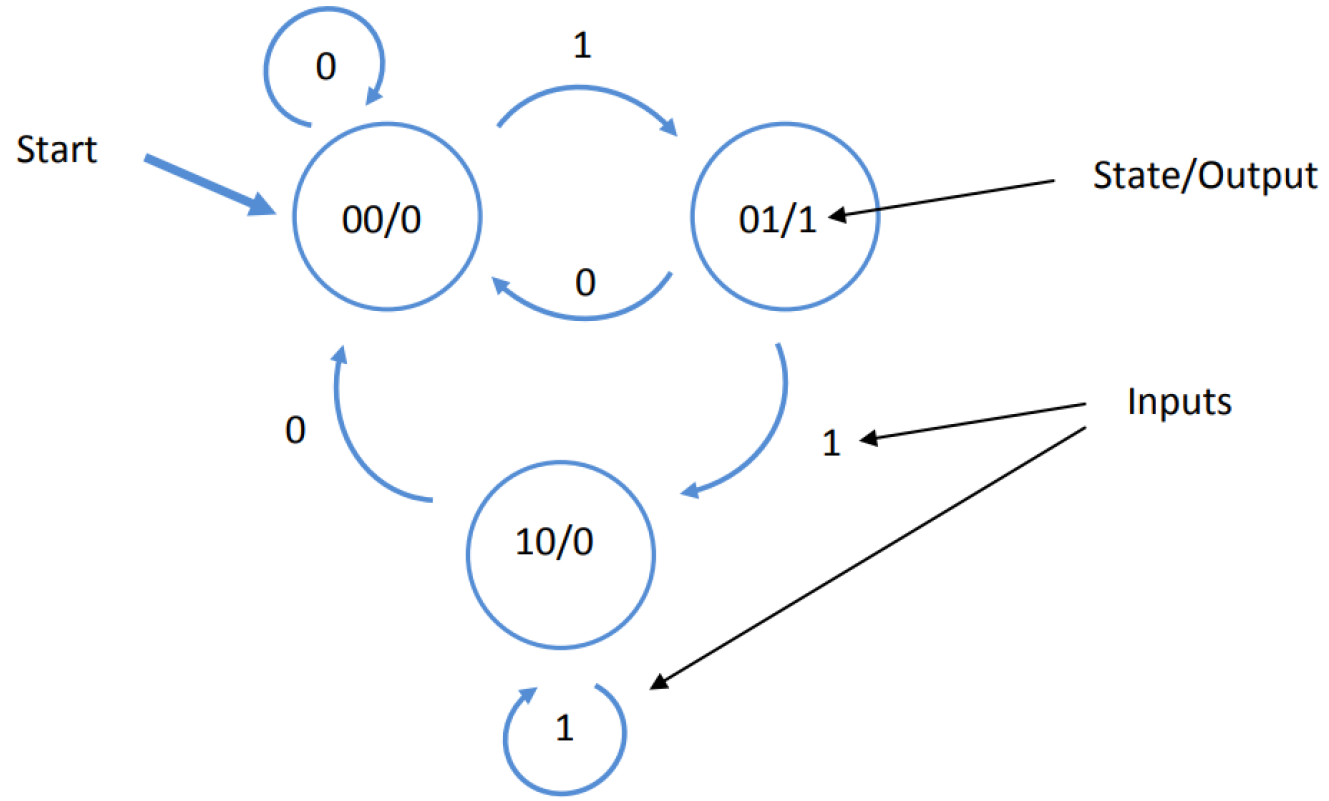
\includegraphics[width=0.8\textwidth]{Graficos3/3a_fsm.png}
    \par\end{centering}
    \caption{Moore state machine diagram}
\end{figure}

Using the diagram, the following table of transitions 
is made.

\begin{figure}[H]
\begin{center}
\begin{tabular}{|c|c|c|c||c|}
    \hline 
    \multicolumn{2}{|c|}{Estado Actual} & \multicolumn{2}{c||}{Estado Siguiente} & \multicolumn{1}{c|}{Salidas}\tabularnewline
    \hline 
    \hline 
    \multirow{2}{*}{} & \multirow{2}{*}{y2 - y1} & \multicolumn{2}{c||}{W} & \multirow{2}{*}{Z}\tabularnewline
    \cline{3-4} 
     &  & \multicolumn{1}{c|}{0} & \multicolumn{1}{c||}{1} & \tabularnewline
    \hline 
    A & 00 & A & B & 0\tabularnewline
    \hline 
    B & 01 & A & C & 1\tabularnewline
    \hline 
    C & 10 & A & C & 0\tabularnewline
    \hline 
    \end{tabular}
    \caption{Moore state machine - Transitions}
\end{center}
\end{figure}
With the transitions, using Karnaugh's maps, the 
functions for the states and the output are made
as shown below.

\begin{figure}[H]
    \begin{center}
         \begin{Karnaughvuit}
            \minterms{5,6}
             \maxterms{0,1,2,4}
             \indeterminats{3,7}
            \implicant{7}{6}{red}
            \implicant{5}{7}{green}
         \end{Karnaughvuit}
         \begin{Karnaughvuit}
            \minterms{2,4,7}
            \maxterms{0,1,3,5,6}
            \implicantsol{2}{red}
            \implicantsol{4}{green}
            \implicantsol{7}{blue}
         \end{Karnaughvuit}
         \caption{Maps for $Y_2$ (left) and $Y_1$ (right) functions.}
    \end{center}
    \end{figure}
Where $Y_2 = W \cdot y_1 + W \cdot y_2$, and $Y_1 = W \cdot \overline{y_2} \cdot \overline{y_1}$. 
From the transitions table, it is simple to see that $Z = y_1$.
With the functions, the state machine is implemented 
using two D Flip Flops as follows. 

\begin{figure}[H]
    \begin{centering}
    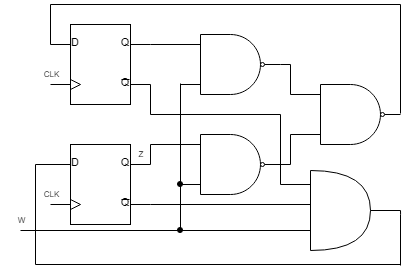
\includegraphics[width=0.8\textwidth]{Graficos3/3a_Compuertas_Moore.png}
    \par\end{centering}
    \caption{Moore state machine - Circuit implementation}
\end{figure}

Now the same system is implemented using a Mealy's 
state machine, wich resulting diagram is shown below.

\begin{figure}[H]
    \begin{centering}
    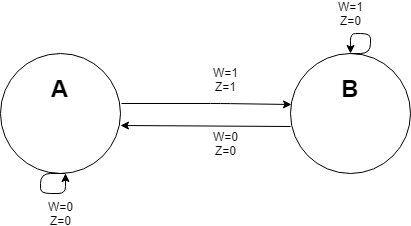
\includegraphics[width=0.8\textwidth]{Graficos3/3b_fsm.png}
    \par\end{centering}
    \caption{Mealy state machine diagram}
\end{figure}

Notice that it requires one less state than Moore's
machine because of the direct connection of the 
from the input to the output. The following 
transition table is made using the diagram.

\begin{figure}[H]
    \begin{center}
        \begin{tabular}{|c|c|c|c||c|c|}
            \hline 
            \multicolumn{2}{|c|}{Estado Actual} & \multicolumn{2}{c||}{Estado Siguiente} & \multicolumn{2}{c|}{Salidas}\tabularnewline
            \hline 
            \hline 
            \multirow{2}{*}{} & \multirow{2}{*}{y} & \multicolumn{2}{c||}{W} & \multicolumn{2}{c|}{Z}\tabularnewline
            \cline{3-6} 
             &  & \multicolumn{1}{c|}{0} & \multicolumn{1}{c||}{1} & W=0 & W=1\tabularnewline
            \hline 
            A & 0 & A & B & 0 & 1\tabularnewline
            \hline 
            B & 1 & A & B & 0 & 0\tabularnewline
            \hline 
            \end{tabular}
        \caption{Mealy state machine - Transitions}
    \end{center}
\end{figure}

With the table, using Karnaugh's maps, are made 
the functions for the states and the output.

\begin{figure}[H]
    \begin{center}
     \begin{Karnaughquatre}
         \minterms{1,3}
        \maxterms{0,2}
        \implicant{1}{3}{red}
     \end{Karnaughquatre}
     \begin{Karnaughquatre}
        \minterms{1}
       \maxterms{0,2,3}
       \implicantsol{1}{red}
    \end{Karnaughquatre}
     \caption{Maps for $Y$ (left) and $Z$ (right)}
    \end{center}
\end{figure}
Where from the left map $Y = W$, and from the right
table $Z = \overline{y} \cdot W$.
With the defined functions, the state machine is 
implemented using one D Flip Flop as shown below.

\begin{figure}[H]
    \begin{centering}
    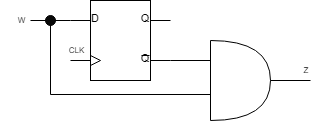
\includegraphics[width=0.8\textwidth]{Graficos3/3b_Compuertas_Mealy.png}
    \par\end{centering}
    \caption{Mealy state machine - Circuit implementation}
\end{figure}

\newpage
Since the internal logic works with 3.3V power supply, 
and the external signals work with 5V, level shifters 
are implemented using BJT transistors. For adapting
the inputs of CLK and W, the circuits are shown 
below. 

\begin{figure}[H]
    \begin{centering}
    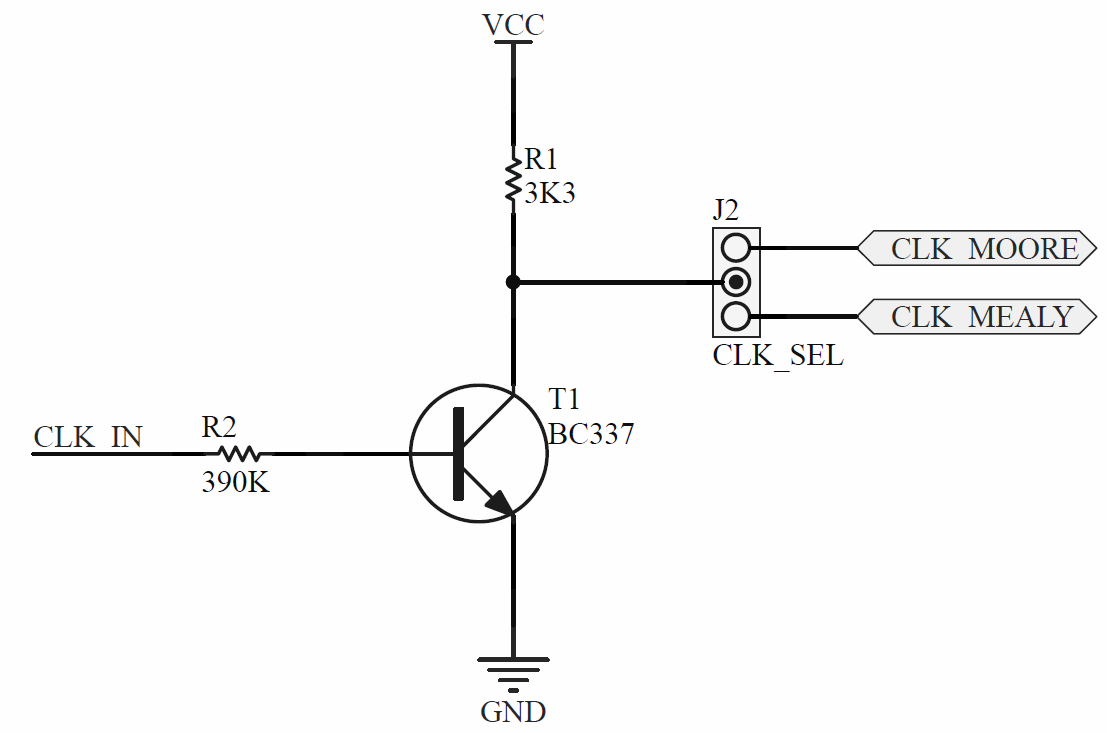
\includegraphics[width=0.45\textwidth]{Graficos3/CLK_Driver.png}
    \par\end{centering}
    \caption{Level shifter for CLK from 5V to 3.3V (VCC)}
\end{figure}

\begin{figure}[H]
    \begin{centering}
    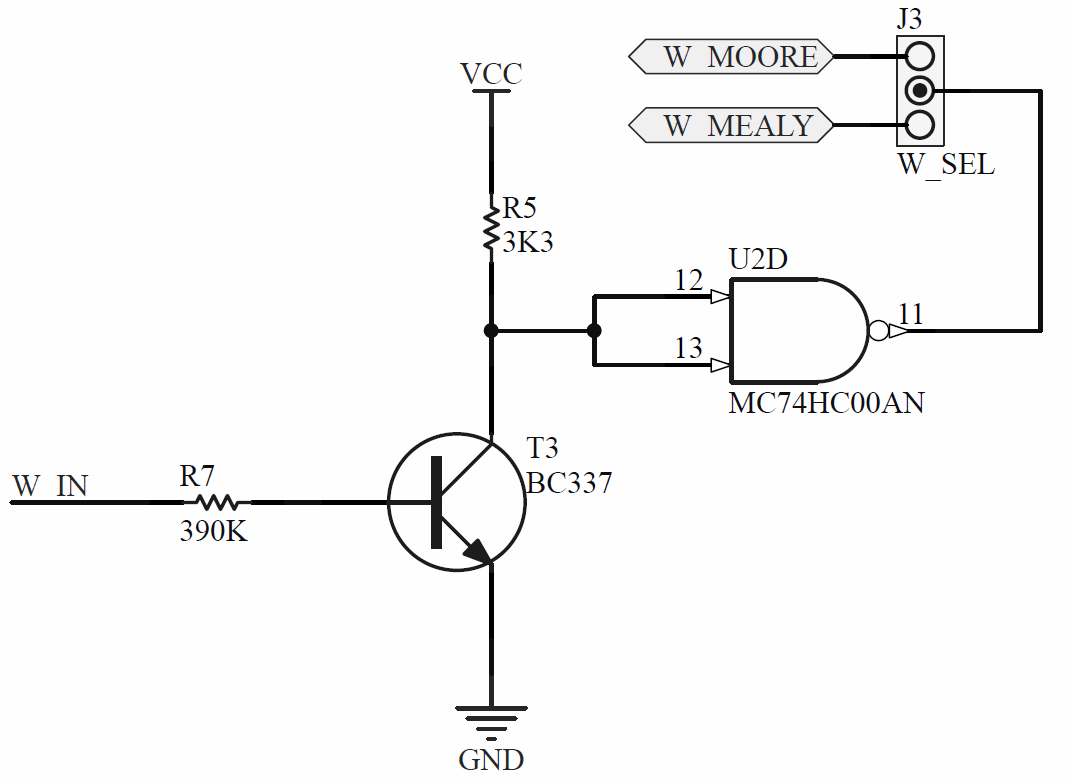
\includegraphics[width=0.45\textwidth]{Graficos3/W_Driver.png}
    \par\end{centering}
    \caption{Level shifter for W from 5V to 3.3V (VCC). The inverting gate is to compense the transistor logic inversion.}
\end{figure}

And for the outputs (Moore and Mealy machines) 
the driver circuit is as shown below.

\begin{figure}[H]
    \begin{centering}
    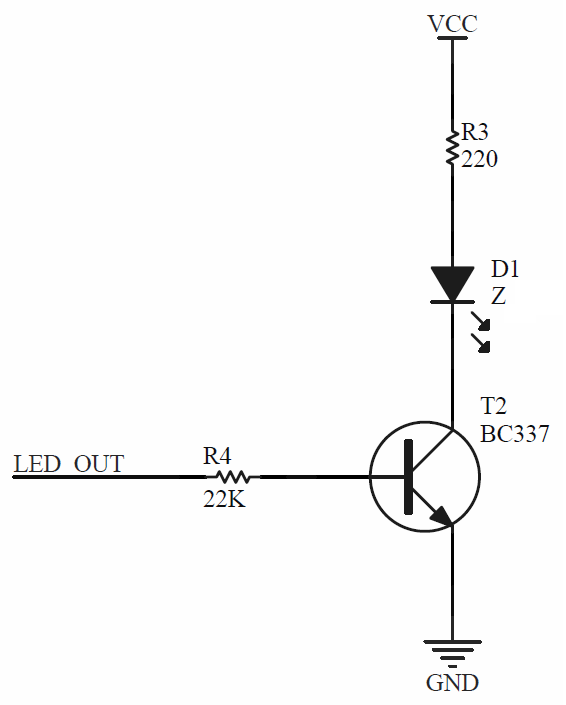
\includegraphics[width=0.3\textwidth]{Graficos3/LED_Driver.png}
    \par\end{centering}
    \caption{Driver for LED output.}
\end{figure}

The design of the circuits with the corresponding 
calculations are included in the $Annex$.

\newpage

\section*{Annex}
\subsection*{Level shifter for inputs}
From the implemented circuit:
\begin{figure}[H]
    \begin{centering}
    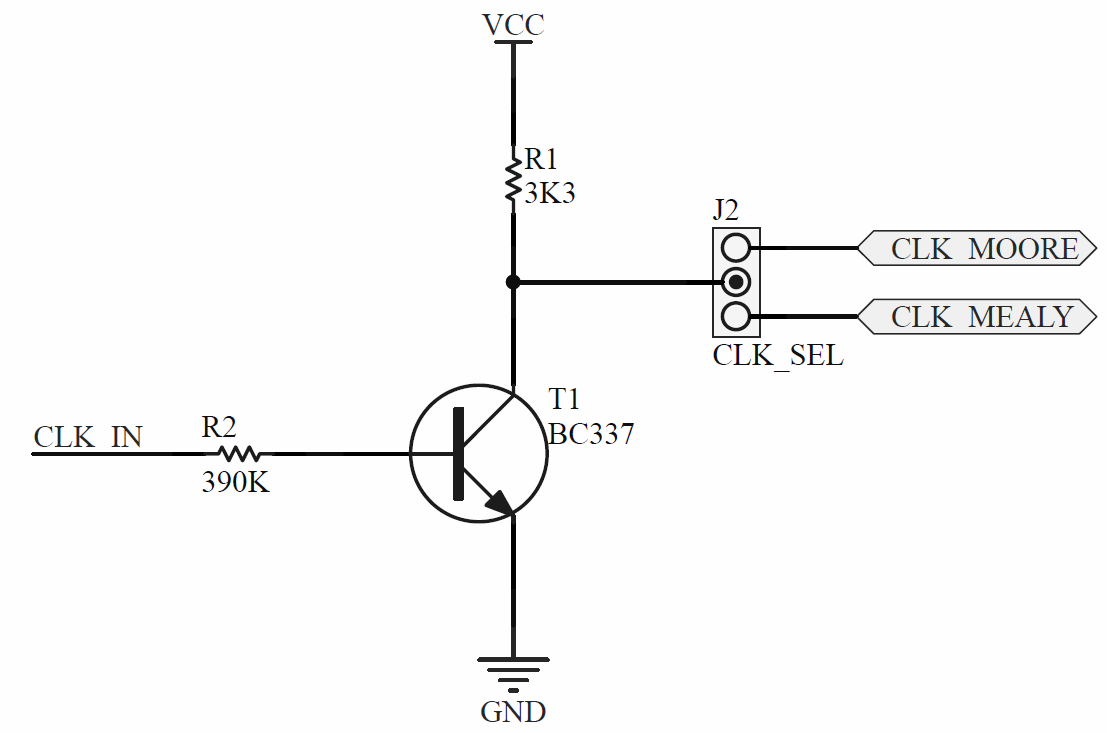
\includegraphics[width=0.5\textwidth]{Graficos3/CLK_Driver.png}
    \par\end{centering}
    \caption{Level shifter for CLK from 5V to 3.3V (VCC)}
\end{figure}

Usign for $I_{SAT} = 1mA$, considerating $VCE_{SAT} = 0.2V$, 
the equation from the out mesh:

$$3.3V - VCE_{SAT} - I_{SAT}R_1 = 0$$
$$\frac{3.3V - VCE_{SAT}}{I_{SAT}} = R_1 = 3.1K\Omega$$
Normalizing we have $R_1 = 3.3K\Omega$.
Considering $HFE_{MIN} = 100$, from the input mesh:

$$5V - VBE_{ON} - \frac{I_C}{HFE_{MIN}}R_2 = 0$$
$$\frac{5V - VBE_{ON}}{I_C}HFE_{MIN} = R_2 = 430K\Omega$$
Normalizing we have $R_2 = 390K\Omega$.

\subsection*{Driver for output led}
Taking the implemented circuit:

\begin{figure}[H]
    \begin{centering}
    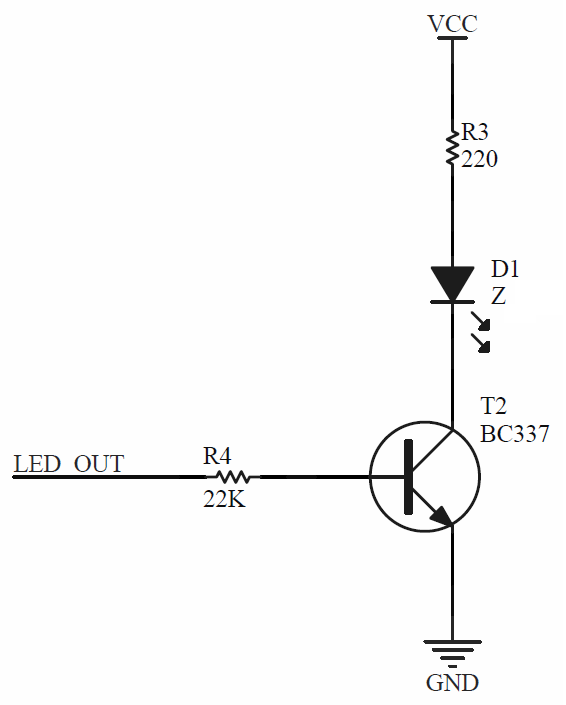
\includegraphics[width=0.3\textwidth]{Graficos3/LED_Driver.png}
    \par\end{centering}
    \caption{Driver for LED output.}
\end{figure}

Usign for $I_{LED} = 10mA$, considerating $VCE_{SAT} = 0.2V$ 
and $V{LED} = 2V$, the equation from the out mesh:

$$3.3V - V_{LED} - VCE_{SAT} - I_{LED}R_3 = 0$$
$$\frac{3.3V - V_{LED} - VCE_{SAT}}{I_{LED}} = R_3 = 110\Omega$$
Normalizing we have $R_3 = 220\Omega$.
Considering $HFE_{MIN} = 100$, from the input mesh:

$$3.3V - VBE_{ON} - \frac{I_C}{HFE_{MIN}}R_4 = 0$$
$$\frac{3.3V - VBE_{ON}}{I_C}HFE_{MIN} = R_4 = 26K\Omega$$
Normalizing we have $R_4 = 22K\Omega$, to guarantee saturation.

\end{document}